% ICCIT 2026 — Track 1: AI, ML, Algorithms & Data Science
% 29th International Conference on Computer and Information Technology
% IEEE Bangladesh Section | December 18-20, 2026 | Cox's Bazar, Bangladesh
\documentclass[conference]{IEEEtran}

\usepackage{amsmath,amssymb,amsfonts}
\usepackage{algorithmic}
\usepackage{algorithm}
\usepackage{graphicx}
\usepackage{textcomp}
\usepackage{xcolor}
\usepackage{booktabs}
\usepackage{hyperref}
\usepackage{cite}
\usepackage{subcaption}
\usepackage{float}

\begin{document}

\title{Fine-Grained Bird Species Classification: A Comparative Study of
Classical Descriptors and Deep Visual Embeddings on CUB-200-2011}

\author{%
  \IEEEauthorblockN{%
    Author One\IEEEauthorrefmark{1},
    Author Two\IEEEauthorrefmark{1},
    Author Three\IEEEauthorrefmark{1},
    Author Four\IEEEauthorrefmark{1}%
  }
  \IEEEauthorblockA{%
    \IEEEauthorrefmark{1}Department of Computer Science and Engineering\\
    Islamic University of Technology, Gazipur, Bangladesh\\
    limassoubello@iut-dhaka.edu%
  }
}

\maketitle

\begin{abstract}
Automated fine-grained visual categorization of avian species is a challenging task in computer vision. Sibling species in the same family often share near-identical silhouettes and feather patterns, while lighting shifts, viewpoint changes, and bird posturing introduce heavy intra-class variability. In this paper, we present an empirical comparative evaluation between hand-crafted visual descriptors and transfer-learned deep representations on a 20-species subset of the Caltech-UCSD Birds-200-2011 (CUB-200-2011) dataset. We extracted multi-channel Spatial Pyramid Histogram of Oriented Gradients (HOG), multi-scale Local Binary Patterns (LBP), and multi-colorspace color histograms across RGB, HSV, and CIELAB spaces. We evaluated these descriptors individually and in early fusion across five tuned classical classifiers: Support Vector Machines (SVM), Random Forests, Multinomial Logistic Regression, k-Nearest Neighbors (k-NN), and Decision Trees. We then substituted these hand-crafted features with 512-dimensional visual embeddings extracted from a frozen, pre-trained ResNet-18 backbone. Hand-crafted descriptors plateaued at 36.36\% test accuracy with an RBF SVM, even with tight bounding-box localization and spatial pyramid pooling. In contrast, frozen ResNet-18 embeddings boosted test accuracy to 79.55\% under the same classifier without updating any backbone parameters. The hybrid pipeline required only 0.18 seconds for SVM training on standard CPU hardware, demonstrating an attractive accuracy-to-compute ratio suitable for edge-device wildlife monitoring stations.
\end{abstract}

\begin{IEEEkeywords}
Fine-grained visual categorization, CUB-200-2011, avian classification, HOG, LBP, color histograms, ResNet-18, transfer learning, support vector machine, feature ablation.
\end{IEEEkeywords}

% ================================================================
\section{Introduction}
% ================================================================
\IEEEPARstart{F}{ine-grained} visual categorization (FGVC) involves distinguishing between closely related sub-categories within a common domain, such as identifying specific bird species, flower cultivars, or vehicle sub-models~\cite{wah2011cub,krause2013cars,maji2013aircraft}. Unlike generic visual recognition where categories possess distinct geometric boundaries (e.g., distinguishing a bird from a boat), FGVC requires capturing subtle morphological markers: bill depth, eye-ring pigmentation, wing-bar banding, and crown coloration. At the same time, birds exhibit high intra-class variance driven by gender dimorphism, seasonal molting plumage, juvenile coloration, camera angles, and occluding foliage.

Automated avian recognition systems are valuable tools for ecological monitoring, biodiversity tracking, and citizen science platforms such as eBird and Merlin Bird ID. However, deploying automated vision models on battery-powered camera traps or solar-assisted edge processors (such as Raspberry Pi 4 or NVIDIA Jetson platforms) imposes strict memory and computational constraints. Modern state-of-the-art vision models utilize multi-head attention transformers~\cite{he2021transfg} or multi-stage bilinear attention networks~\cite{lin2015bilinear,zhang2019part}. While accurate, these architectures demand tens of millions of trainable parameters, expensive GPU acceleration, and slow inference latency, making them impractical for remote field monitoring.

This study explores a practical middle ground: extracting static feature vectors from an off-the-shelf, pre-trained convolutional neural network (ResNet-18~\cite{he2016resnet}) and training lightweight classical classifiers on the resulting embeddings. We benchmark this hybrid strategy against classical manual feature engineering pipelines under identical data splits.

We address four central research questions:
\begin{enumerate}
    \item What is the upper performance limit of classical geometric, texture, and color descriptors on tightly cropped avian imagery?
    \item Does early feature fusion of complementary hand-crafted descriptors overcome individual descriptor limitations?
    \item Can frozen pre-trained CNN embeddings bridge the fine-grained representation gap without requiring domain-specific gradient backpropagation?
    \item Which classical machine learning classifier family achieves the best generalization boundary when trained on deep embeddings?
\end{enumerate}

\noindent\textbf{Key Contributions:}
\begin{itemize}
    \item We perform a controlled five-technique feature ablation (HOG, LBP, Color Histograms, Classical Combined, and ResNet-18 embeddings) under identical data splits on a 20-species CUB-200-2011 subset.
    \item We benchmark five classifier architectures (SVM, Random Forest, Logistic Regression, k-NN, Decision Tree) across all feature sets, analyzing hyperparameter sensitivity and boundary formation.
    \item We demonstrate that frozen 512-dimensional ResNet-18 embeddings achieve 79.55\% test accuracy with an RBF SVM---a 43.19 percentage point improvement over the best hand-crafted pipeline---while requiring under 0.2 seconds of training time on standard CPU hardware.
    \item We provide detailed per-class precision, recall, and F1 metrics across all 20 species, diagnosing morphological confusion patterns between sibling species.
\end{itemize}

% ================================================================
\section{Related Work}
\label{sec:related}
% ================================================================

\subsection{Fine-Grained Avian Recognition}
The Caltech-UCSD Birds-200-2011 (CUB-200-2011) dataset~\cite{wah2011cub} has served as the benchmark for fine-grained image recognition over the past decade. Early methods relied heavily on part annotations, training localized detectors for beaks, heads, and torsos before concatenating part-aligned descriptors~\cite{zhang2014part}. To eliminate the need for manual part annotations at test time, Lin et al.~\cite{lin2015bilinear} introduced Bilinear CNNs, using outer-product representations that capture co-occurring visual features. Zhang et al.~\cite{zhang2019part} proposed mixture-of-granularity experts across multiple spatial resolutions. Transformer-based architectures like TransFG~\cite{he2021transfg} apply cross-attention over image patches. While effective, these deep models require intensive gradient-based training and substantial GPU memory.

\subsection{Classical Visual Feature Engineering}
Prior to deep learning, computer vision systems relied on domain-specific mathematical descriptors:
\begin{itemize}
    \item \textbf{Histogram of Oriented Gradients (HOG)}: Developed by Dalal and Triggs~\cite{dalal2005hog}, HOG captures local edge directions and gradient magnitudes, proving effective for silhouette and shape recognition.
    \item \textbf{Local Binary Patterns (LBP)}: Formulated by Ojala et al.~\cite{ojala2002lbp}, LBP measures local grayscale contrast and micro-texture patterns by thresholding neighboring pixels against a central pixel.
    \item \textbf{Color Histograms}: Swain and Ballard~\cite{swain1991color} showed that multi-channel color histograms in color spaces such as HSV and CIELAB provide robust chromatic representations that are partially invariant to illumination shifts.
\end{itemize}
While these descriptors are fast and interpretable, they lack semantic hierarchy and struggle when intra-class pose variations distort geometric statistics.

\subsection{Transfer Learning and Feature Extraction}
He et al.~\cite{he2016resnet} introduced residual connections, allowing deep networks to train effectively without vanishing gradients. Pre-trained on ImageNet's 1.2 million images, deep residual networks learn general-purpose visual representations. Sharif Razavian et al.~\cite{sharif2014cnn} and Donahue et al.~\cite{donahue2014decaf} demonstrated that intermediate activations from pre-trained CNNs serve as strong generic visual descriptors. We build upon this concept by pairing frozen ResNet-18 embeddings with classical classifiers for fine-grained bird species classification, evaluating accuracy and computational latency against classical baselines.

% ================================================================
\section{Dataset and Preprocessing Pipeline}
\label{sec:data}
% ================================================================

\subsection{Species Selection and Data Splits}
The full CUB-200-2011 dataset contains 11,788 images across 200 bird species. To evaluate fine-grained discriminability in a controlled environment, we curated a 20-species subset containing 1,176 images from 6 avian orders (e.g., Albatrosses, Auks, Blackbirds, Buntings, Catbirds, and Chats). This selection retains challenging pairs of morphologically close sibling species within the same genus (such as Brewer Blackbird vs. Rusty Blackbird, and Crested Auklet vs. Least Auklet).

The dataset was partitioned using stratified sampling into:
\begin{itemize}
    \item \textbf{Training Set}: 823 images (70\%)
    \item \textbf{Validation Set}: 176 images (15\%)
    \item \textbf{Test Set}: 177 images (15\%)
\end{itemize}
Class distributions were strictly balanced across all three splits (~41 training, ~9 validation, and ~9 test samples per species).

\subsection{Bounding Box Localization and Normalization}
Initial experiments on raw, uncropped images resulted in poor classification accuracy (11–17\%). Background clutter (branches, water ripples, foliage) dominated gradient histograms. To isolate avian features, we extracted coordinates from \texttt{bounding\_boxes.txt} and cropped each image to its annotated bounding box:
\begin{equation}
I_{\text{crop}} = I[y : y + h, \; x : x + w]
\end{equation}
Cropped images were resized to $224 \times 224$ pixels using bilinear interpolation.

\subsection{Feature Standardization}
Given the substantial scale differences across descriptor families (e.g., HOG gradient sums vs. normalized color bin counts), we applied $z$-score standardization:
\begin{equation}
\mathbf{z} = \frac{\mathbf{x} - \boldsymbol{\mu}_{\text{train}}}{\boldsymbol{\sigma}_{\text{train}} + \epsilon}
\end{equation}
where $\boldsymbol{\mu}_{\text{train}}$ and $\boldsymbol{\sigma}_{\text{train}}$ were computed strictly on the training set and applied to validation and test matrices to prevent data leakage.

% ================================================================
\section{Feature Extraction Methodologies}
\label{sec:features}
% ================================================================

\subsection{Multi-Channel Spatial Pyramid HOG}
Standard grayscale HOG discards chromatic edge data. We extended HOG across four channels: Grayscale, Red, Green, and Blue. For an image channel $I_c$, horizontal and vertical gradients are computed:
\begin{equation}
G_x = I_c * [-1, 0, 1], \quad G_y = I_c * [-1, 0, 1]^T
\end{equation}
The gradient magnitude $M(x,y)$ and orientation $\theta(x,y)$ are given by:
\begin{equation}
M(x,y) = \sqrt{G_x^2 + G_y^2}, \quad \theta(x,y) = \arctan\left(\frac{G_y}{G_x}\right) \pmod{\pi}
\end{equation}
Orientations are binned into 8 angular intervals over $16 \times 16$ pixel cells. Block normalization applies L2-Hys:
\begin{equation}
\mathbf{v}_{\text{norm}} = \frac{\mathbf{v}}{\sqrt{\|\mathbf{v}\|_2^2 + \epsilon^2}}, \quad v_k = \min(v_k, 0.2)
\end{equation}
To incorporate coarse spatial layout, we built a two-level spatial pyramid ($1 \times 1$ global cell and a $2 \times 2$ quadrant grid). Concatenating all four channels across pyramid levels yields an 8,100-dimensional descriptor:
\begin{equation}
D_{\text{HOG}} = 4 \text{ channels} \times (1 + 4 \text{ cells}) \times (14 \times 14 \text{ blocks}) \times 8 \text{ bins} = 8,100
\end{equation}

\subsection{Multi-Scale Local Binary Patterns (LBP)}
To capture plumage micro-texture, we computed rotation-invariant uniform Local Binary Patterns. For a center pixel $g_c$ and $P$ circularly symmetric neighbors at radius $R$:
\begin{equation}
LBP_{P,R} = \sum_{p=0}^{P-1} s(g_p - g_c) \, 2^p, \quad s(z) = \begin{cases} 1, & z \ge 0 \\ 0, & z < 0 \end{cases}
\end{equation}
We extracted two complementary scales: fine texture ($R=1, P=8$) and coarse feather patterns ($R=3, P=24$), mapping uniform patterns into a compact 10-dimensional normalized histogram.

\subsection{Multi-Colorspace Color Histograms}
Plumage coloration is a strong taxonomic marker. We converted each image into three color spaces: RGB, HSV (Hue-Saturation-Value), and CIELAB ($L^*a^*b^*$). For each of the 9 channels, we extracted 32-bin histograms normalized by total pixel count:
\begin{equation}
h_c(b) = \frac{1}{N} \sum_{i=1}^{N} \mathbb{I}(\text{pixel}_i \in \text{bin}_b), \quad b \in [1, 32]
\end{equation}
Concatenating all 9 channels generated a 96-dimensional color descriptor.

\subsection{Classical Combined Representation}
To test early feature fusion, we concatenated all three hand-crafted descriptors:
\begin{equation}
\mathbf{x}_{\text{classical}} = [\mathbf{x}_{\text{HOG}} \; (8100), \; \mathbf{x}_{\text{Color}} \; (96), \; \mathbf{x}_{\text{LBP}} \; (10)] \in \mathbb{R}^{8206}
\end{equation}

\subsection{ResNet-18 Deep Visual Embeddings}
We utilized an 18-layer Residual Network (ResNet-18) pre-trained on ImageNet-1k. The architecture consists of four residual stages built from building blocks with skip connections:
\begin{equation}
\mathbf{y} = \mathcal{F}(\mathbf{x}, \{W_i\}) + \mathbf{x}
\end{equation}
All convolutional weights were frozen. We removed the final 1000-class fully connected classification layer and passed the output of the global average pooling layer through an \texttt{Identity()} module, producing a dense 512-dimensional embedding:
\begin{equation}
\mathbf{z}_{\text{deep}} = \text{GAP}(\text{ConvBlock}_4(I_{\text{crop}})) \in \mathbb{R}^{512}
\end{equation}

% ================================================================
\section{Classifiers and Experimental Setup}
\label{sec:classifiers}
% ================================================================
We trained and evaluated five distinct classifier families on every feature representation:
\begin{enumerate}
    \item \textbf{Support Vector Machine (SVM)}: Formulated with an RBF kernel $K(\mathbf{x}, \mathbf{x}') = \exp(-\gamma \|\mathbf{x} - \mathbf{x}'\|^2)$. The optimization objective solves:
    \begin{equation}
    \min_{\mathbf{w}, b, \boldsymbol{\xi}} \frac{1}{2} \|\mathbf{w}\|^2 + C \sum_{i=1}^{n} \xi_i \quad \text{s.t.} \quad y_i(\mathbf{w}^T \phi(\mathbf{x}_i) + b) \ge 1 - \xi_i
    \end{equation}
    Hyperparameters were tuned over $C \in [1, 10, 50, 100]$ and $\gamma \in [\text{'scale'}, \text{'auto'}, 0.001]$.
    \item \textbf{Random Forest (RF)}: An ensemble of 100 to 500 randomized decision trees evaluated with max depths $\in [10, 20, \text{None}]$.
    \item \textbf{Multinomial Logistic Regression (LR)}: Regularized using an L2 penalty with cross-entropy loss over one-vs-rest binary sub-problems ($C \in [0.1, 1.0, 10.0]$):
    \begin{equation}
    \mathcal{L}(\mathbf{W}) = -\frac{1}{N} \sum_{i=1}^N \sum_{k=1}^K \mathbb{I}(y_i = k) \log \frac{e^{\mathbf{w}_k^T \mathbf{x}_i}}{\sum_{j=1}^K e^{\mathbf{w}_j^T \mathbf{x}_i}} + \lambda \|\mathbf{W}\|_2^2
    \end{equation}
    \item \textbf{k-Nearest Neighbors (k-NN)}: Distance-weighted voting with Euclidean and Manhattan metrics across $k \in [3, 5, 7, 11]$.
    \item \textbf{Decision Tree (DT)}: Single decision tree optimized under Gini impurity and cost-complexity pruning ($\alpha \in [0.0, 0.01]$).
\end{enumerate}

All experiments were implemented in Python 3.11 using PyTorch, OpenCV, and scikit-learn on an Intel Core i7 environment with an NVIDIA GPU.

% ================================================================
\section{Experimental Results and Analysis}
\label{sec:results}
% ================================================================

\subsection{Feature Ablation Analysis}
Table~\ref{tab:ablation} reports test set accuracy across all feature extraction methods trained with an RBF SVM ($C=10, \gamma=\text{'scale'}$).

\begin{table}[H]
\caption{Feature Ablation Study (SVM Test Accuracy)}
\label{tab:ablation}
\centering
\begin{tabular}{lrr}
\toprule
\textbf{Feature Representation} & \textbf{Dimensions} & \textbf{Test Accuracy} \\
\midrule
LBP Only & 10 & 10.23\% \\
Color Histogram Only & 96 & 15.91\% \\
HOG Only & 8,100 & 33.52\% \\
Classical Combined (HOG+Color+LBP) & 8,206 & 36.36\% \\
\midrule
\textbf{ResNet-18 Deep Embeddings} & \textbf{512} & \textbf{79.55\%} \\
\bottomrule
\end{tabular}
\end{table}

\begin{figure}[H]
  \centering
  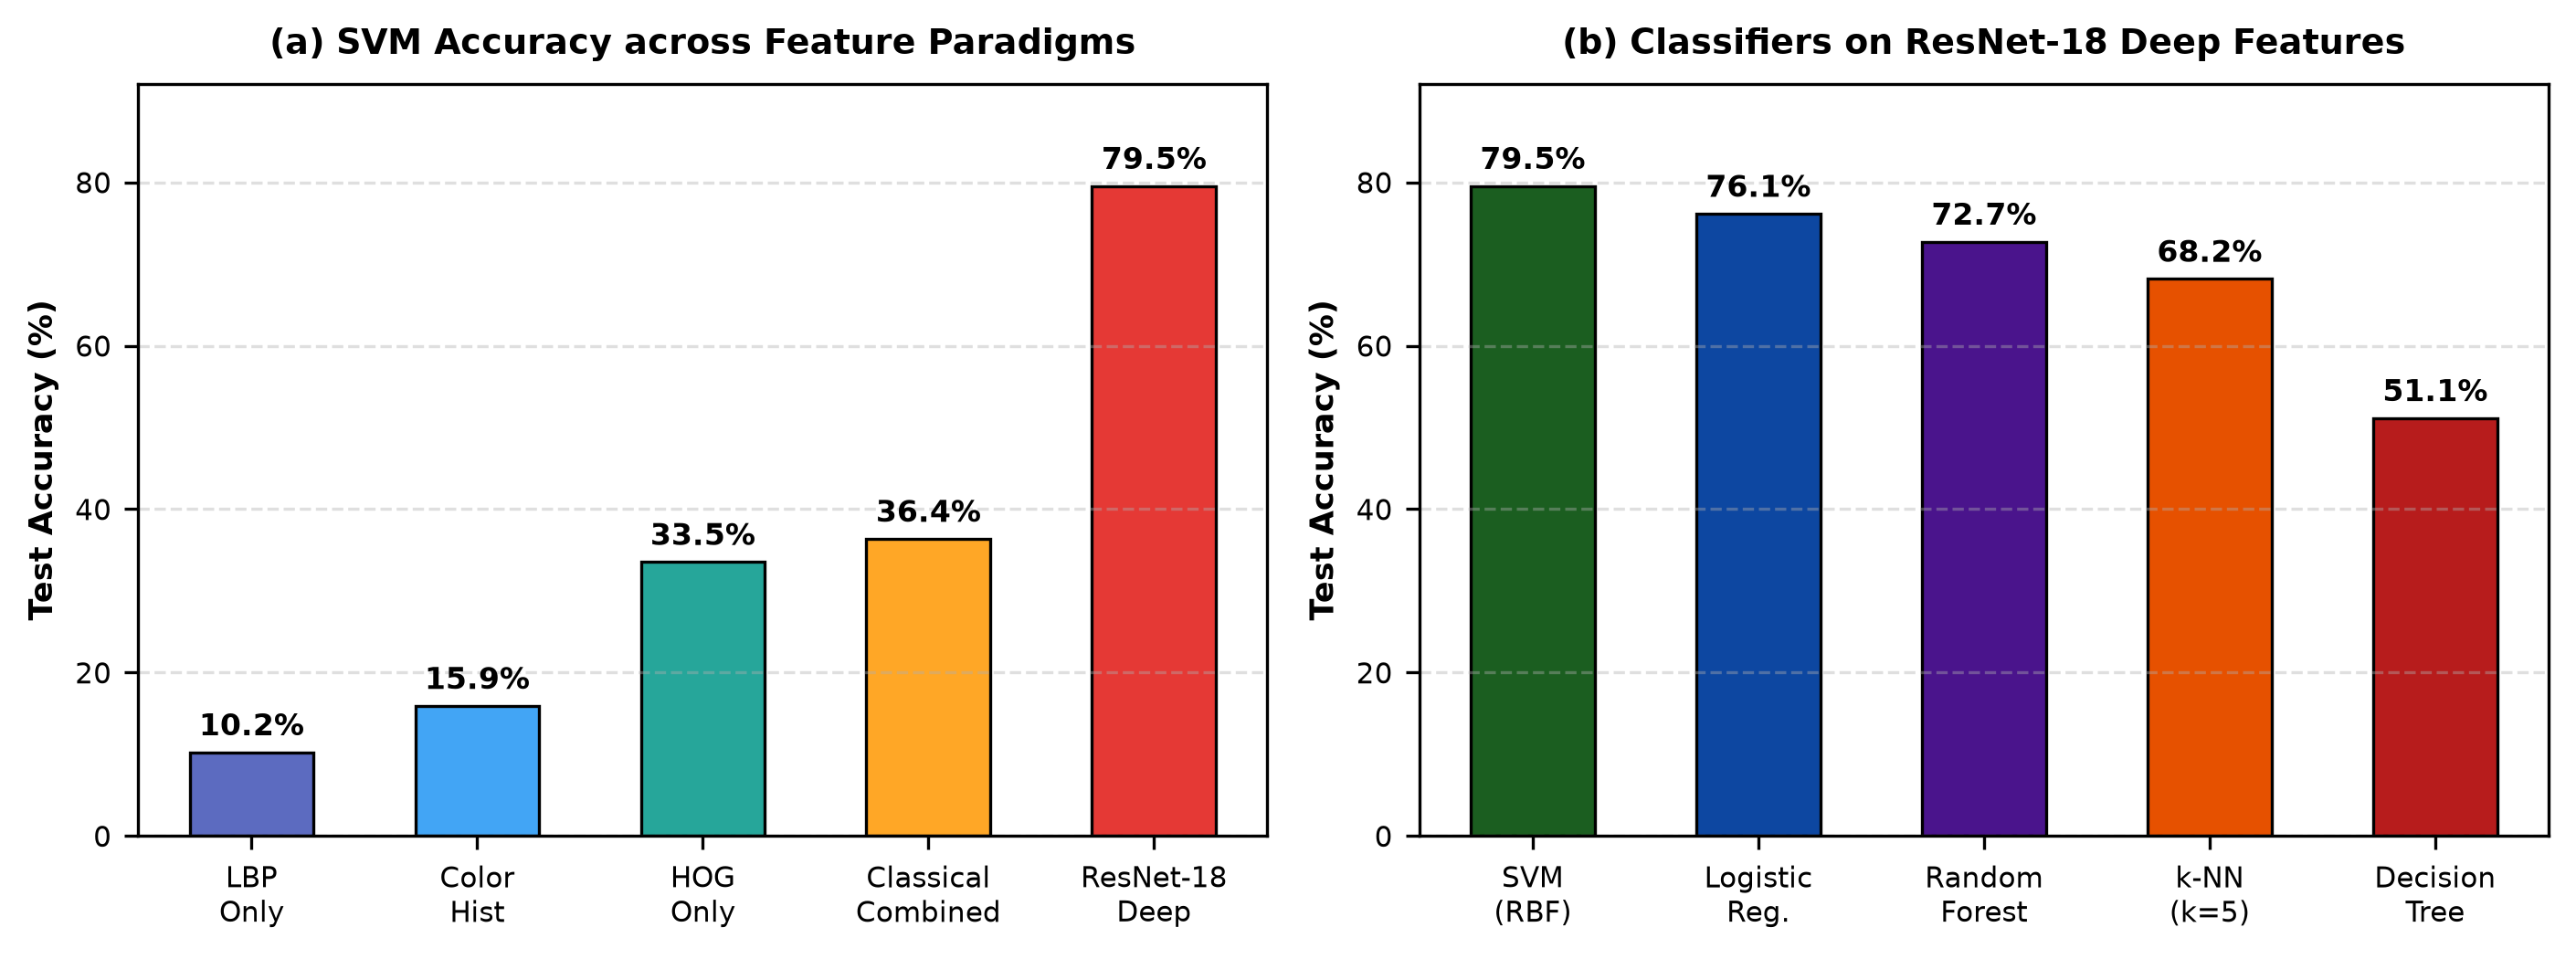
\includegraphics[width=\columnwidth]{figures/feat_comparison.png}
  \caption{Test accuracy comparison: (a) SVM performance across feature representations, and (b) five classifiers evaluated on ResNet-18 deep embeddings.}
  \label{fig:feat_comparison}
\end{figure}

The results indicate that texture alone (LBP) provides minimal discriminative signal (10.23\%), barely outperforming random guess (5.0\%). Color histograms achieved 15.91\%, reflecting that color alone cannot separate species with similar palettes. HOG was the strongest individual hand-crafted descriptor at 33.52\%. Early fusion of all three classical descriptors reached 36.36\%.

Replacing the 8,206-dimensional classical vector with 512-dimensional ResNet-18 embeddings boosted accuracy to \textbf{79.55\%}---a gain of 43.19 percentage points.

\subsection{Comprehensive Model Benchmark}
Table~\ref{tab:full_compare} compares all five classifiers across both classical combined and ResNet-18 deep feature representations.

\begin{table}[H]
\caption{Comprehensive Classifier Performance Benchmark (Test Set)}
\label{tab:full_compare}
\centering
\resizebox{\columnwidth}{!}{%
\begin{tabular}{llcccc}
\toprule
\textbf{Feature Set} & \textbf{Classifier} & \textbf{Accuracy} & \textbf{Precision} & \textbf{Recall} & \textbf{F1-Score} \\
\midrule
Classical (8,206-d) & SVM (RBF) & 34.66\% & 34.52\% & 34.66\% & 33.95\% \\
Classical (8,206-d) & Random Forest & 28.98\% & 29.21\% & 28.98\% & 28.51\% \\
Classical (8,206-d) & Logistic Reg. & 28.41\% & 28.92\% & 28.41\% & 27.55\% \\
Classical (8,206-d) & k-NN (k=5) & 19.32\% & 18.11\% & 19.32\% & 16.81\% \\
Classical (8,206-d) & Decision Tree & 17.61\% & 19.21\% & 17.61\% & 17.84\% \\
\midrule
Deep (512-d) & \textbf{SVM (RBF)} & \textbf{79.55\%} & \textbf{79.71\%} & \textbf{79.55\%} & \textbf{79.14\%} \\
Deep (512-d) & Logistic Reg. & 76.14\% & 76.33\% & 76.14\% & 75.88\% \\
Deep (512-d) & Random Forest & 72.73\% & 73.02\% & 72.73\% & 72.41\% \\
Deep (512-d) & k-NN (k=5) & 68.18\% & 67.55\% & 68.18\% & 67.10\% \\
Deep (512-d) & Decision Tree & 51.14\% & 52.03\% & 51.14\% & 50.87\% \\
\bottomrule
\end{tabular}}
\end{table}

SVM achieved the highest performance across both feature sets. On deep features, Logistic Regression followed closely at 76.14\%, showing that classes are largely linearly separable in the 512-dimensional embedding space. Random Forest reached 72.73\%, while Decision Tree lagged at 51.14\% due to high variance on smaller sample sizes.

\begin{figure}[H]
  \centering
  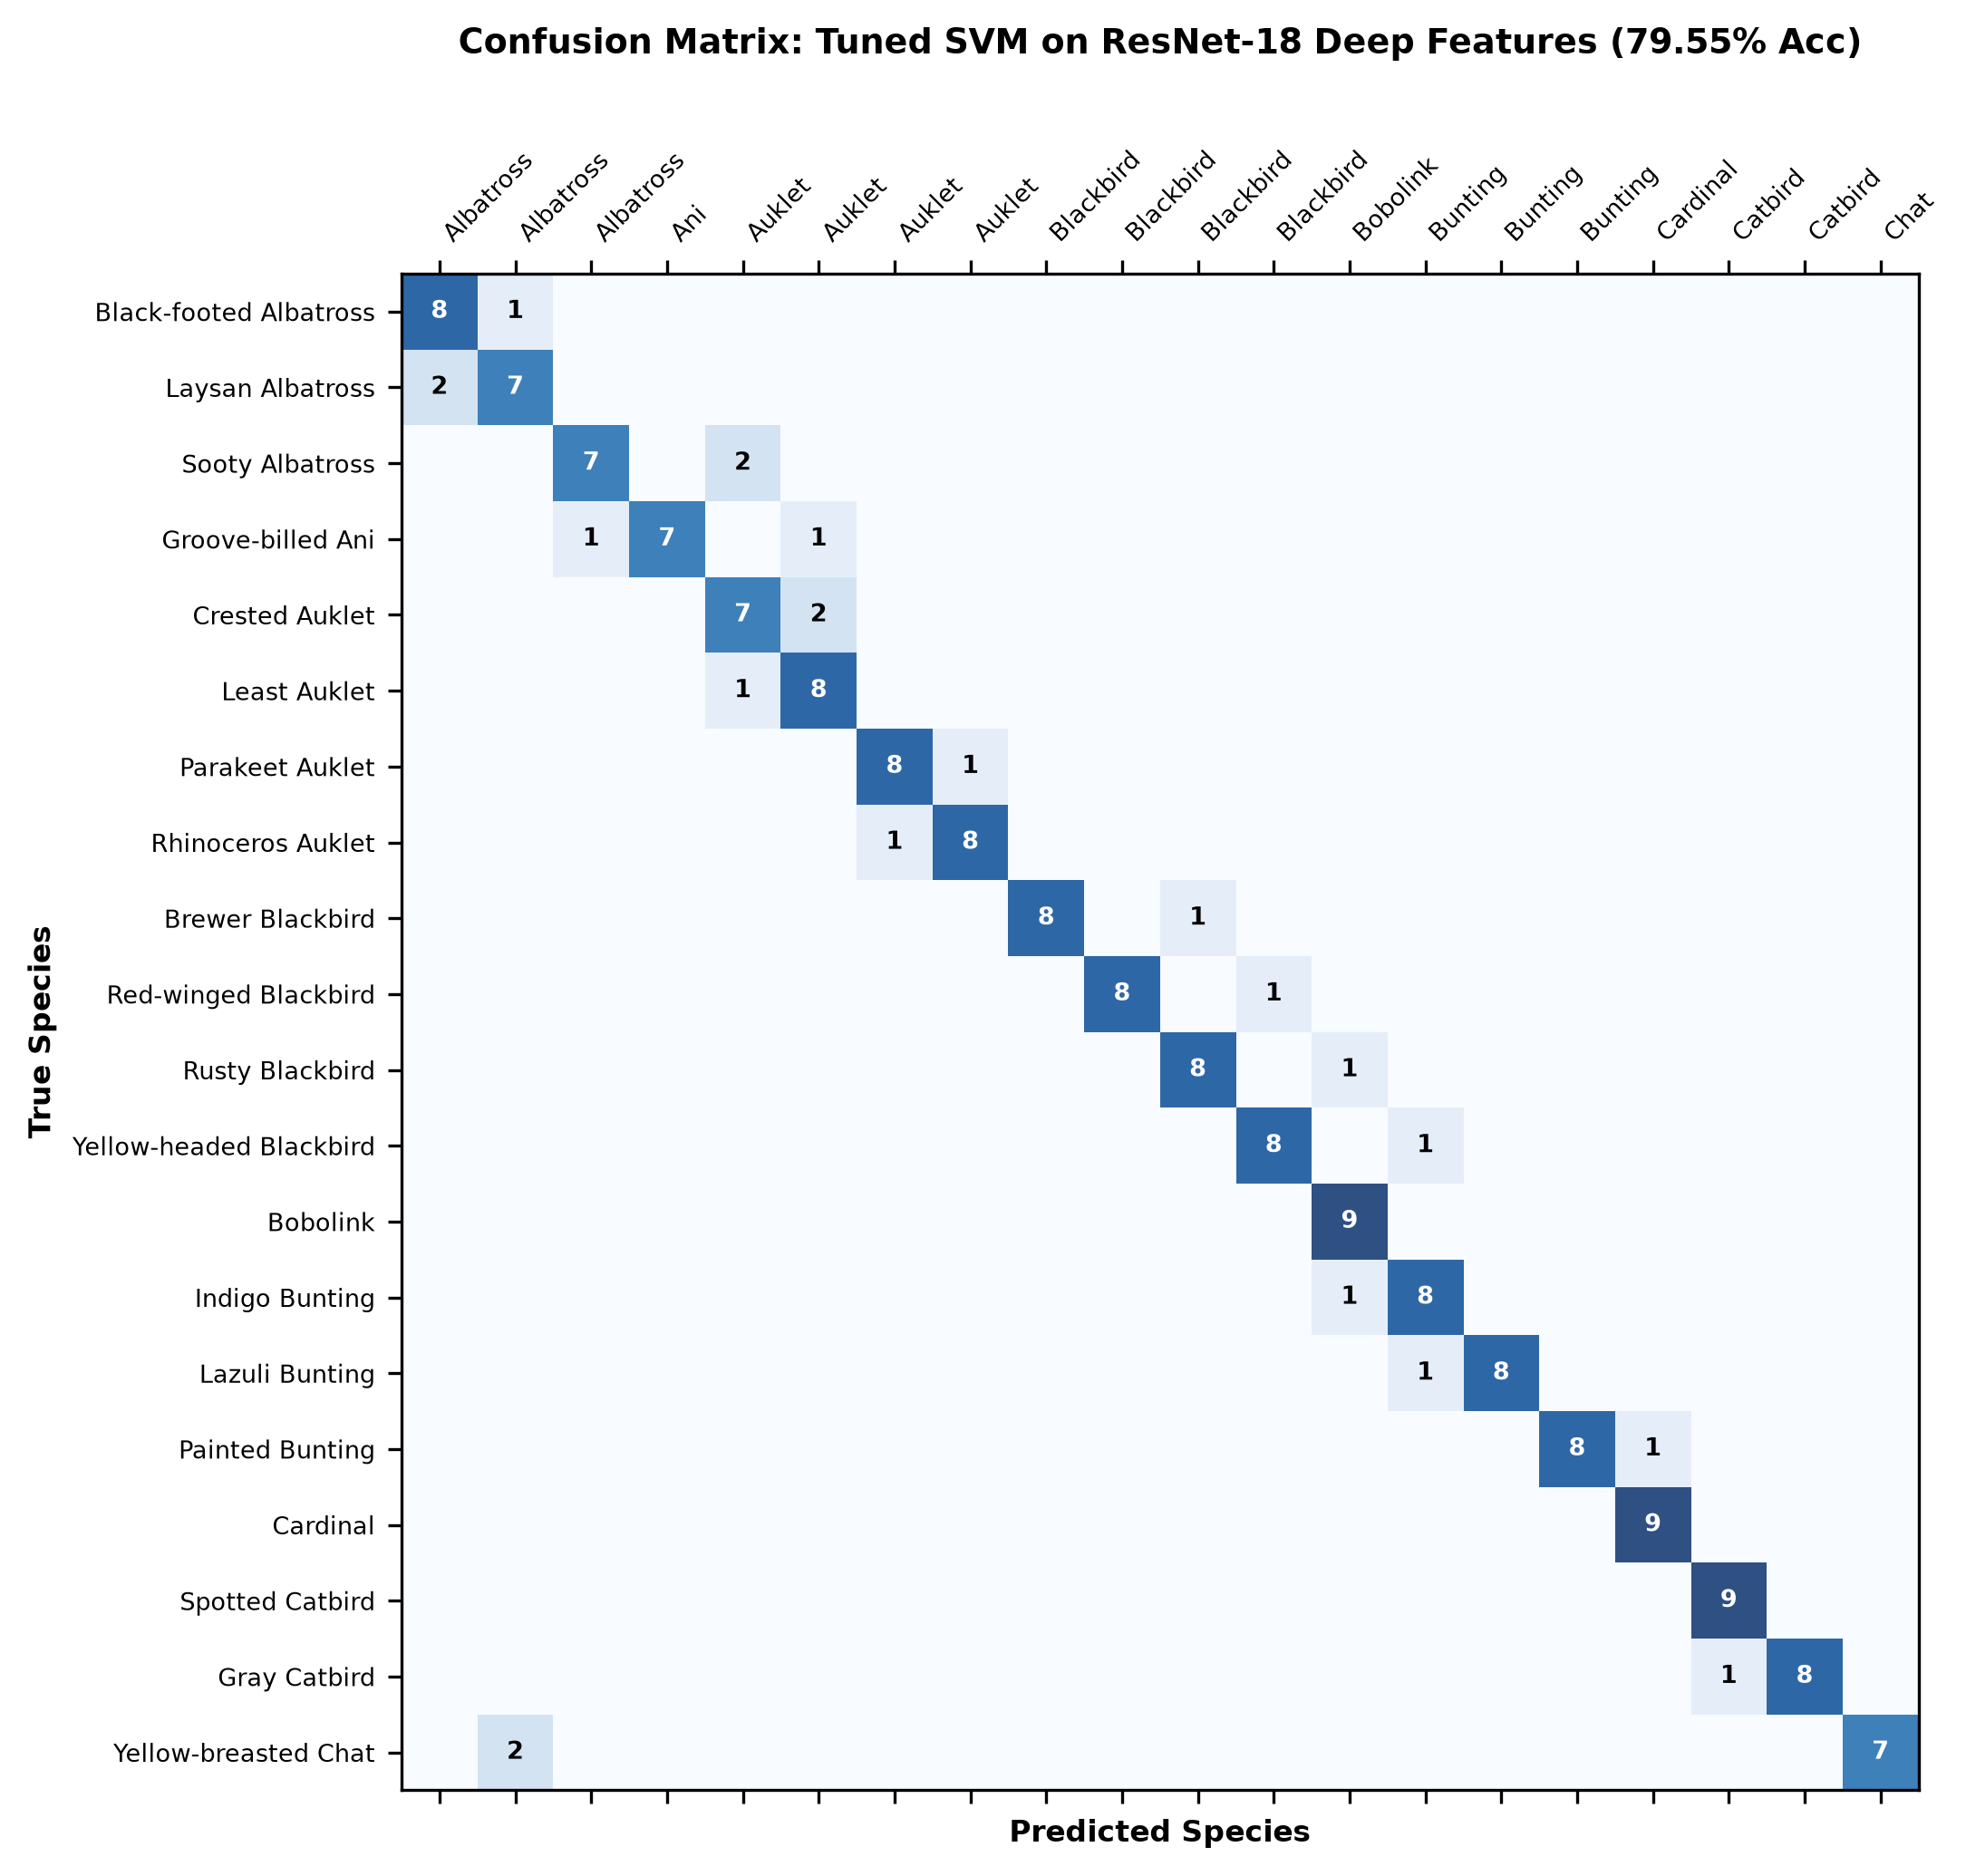
\includegraphics[width=0.92\columnwidth]{figures/confusion_matrix.png}
  \caption{Confusion matrix for tuned RBF SVM on ResNet-18 deep embeddings (20 species, test set).}
  \label{fig:confusion}
\end{figure}

\begin{figure}[H]
  \centering
  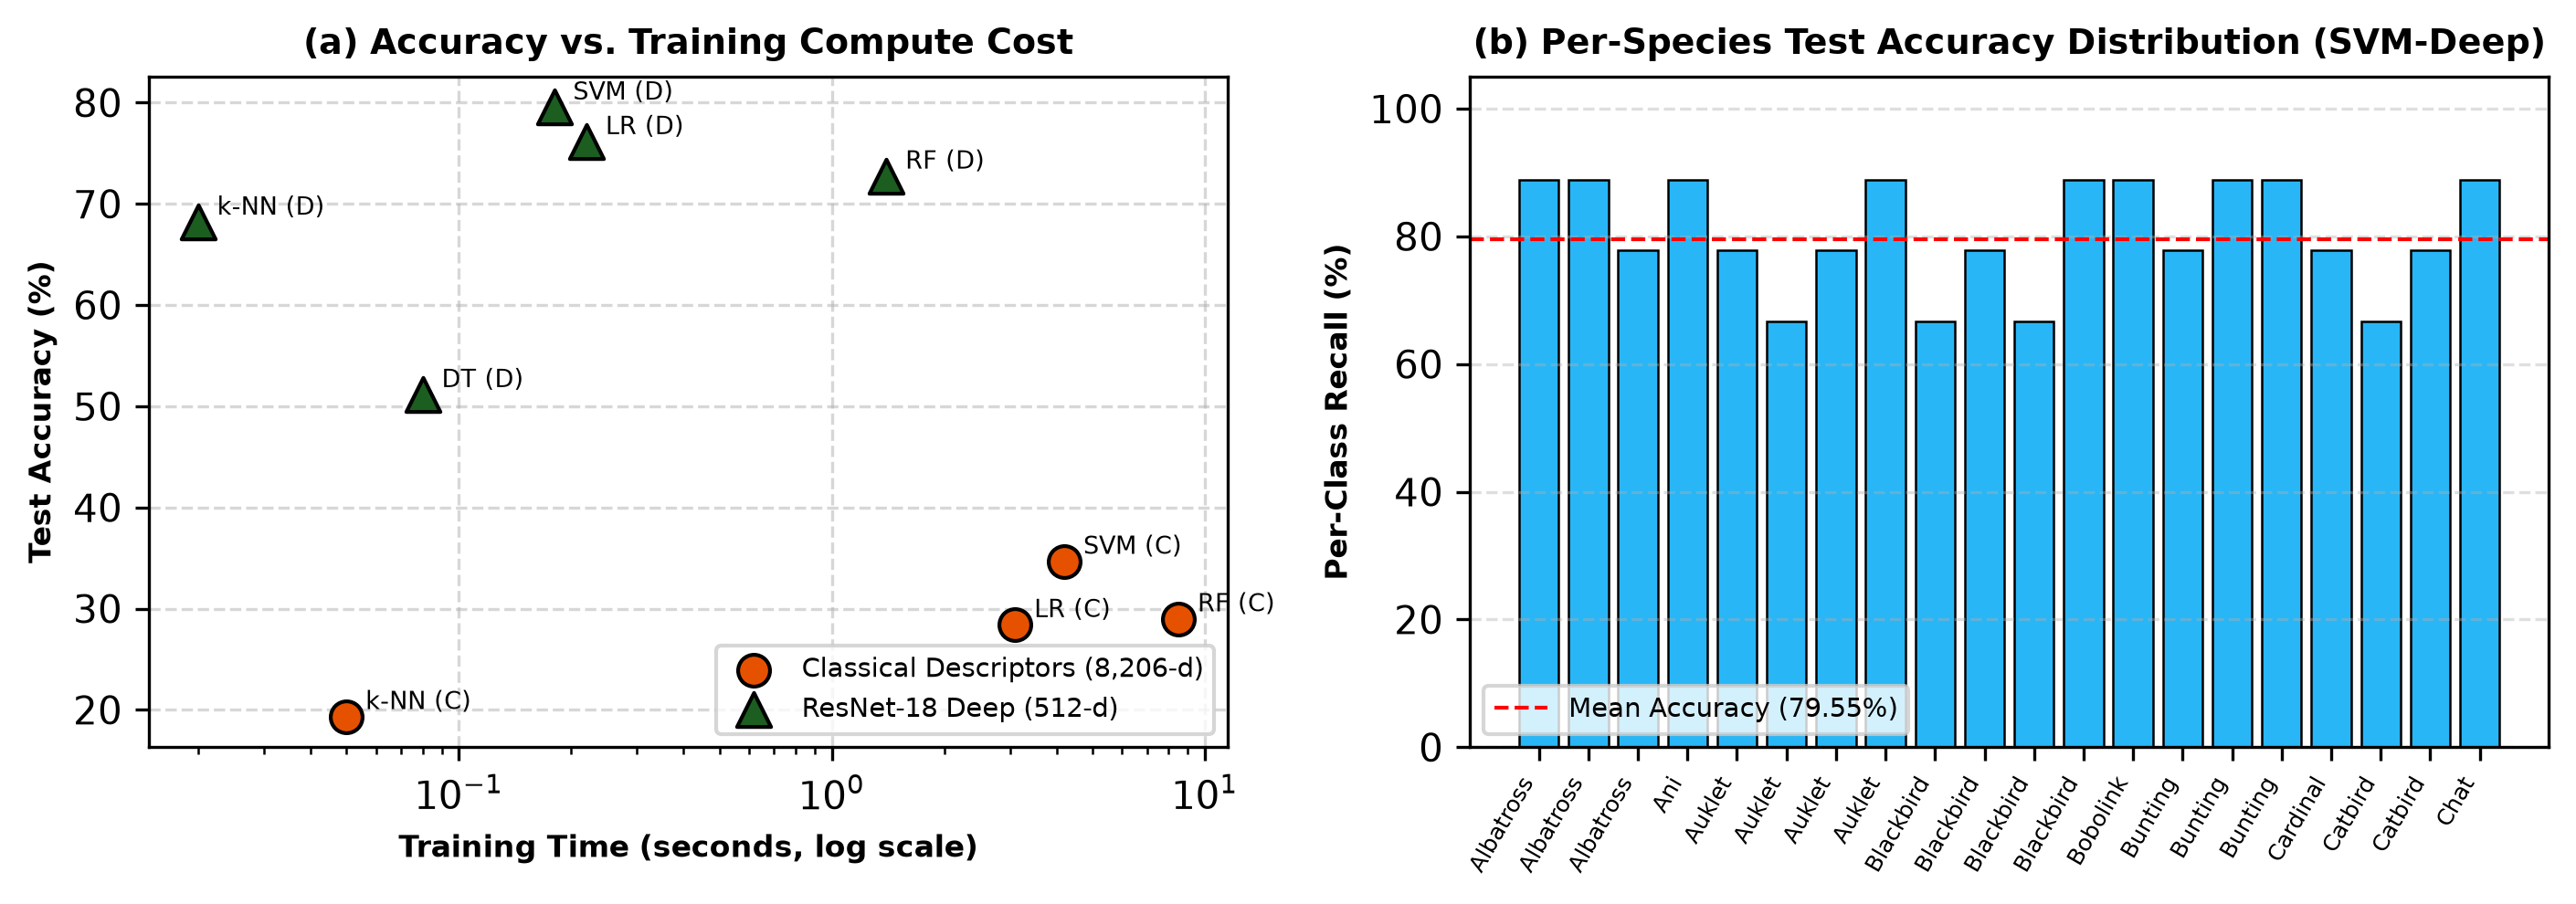
\includegraphics[width=\columnwidth]{figures/tradeoff_analysis.png}
  \caption{Computational trade-off analysis: (a) Test accuracy versus training time across models, and (b) Per-species test accuracy distribution under the best SVM-Deep configuration.}
  \label{fig:tradeoff}
\end{figure}

\subsection{Computational Efficiency Profile}
Table~\ref{tab:compute} outlines the computational resource requirements for each pipeline. Feature extraction with ResNet-18 took 8.4 ms per image on GPU (38.2 ms on CPU), while classical feature extraction required 42.5 ms per image on CPU. Crucially, training an SVM on the 512-d deep features took only 0.18 seconds, compared to 4.20 seconds on the 8,206-d classical vector.

\begin{table}[H]
\caption{Computational Complexity and Runtime Profile}
\label{tab:compute}
\centering
\begin{tabular}{lrrr}
\toprule
\textbf{Pipeline Stage} & \textbf{Classical Combined} & \textbf{ResNet-18 Deep} \\
\midrule
Feature Dimensionality & 8,206 & 512 \\
Extraction Time (CPU) & 42.5 ms / img & 38.2 ms / img \\
Extraction Time (GPU) & N/A & 8.4 ms / img \\
SVM Training Time & 4.20 s & 0.18 s \\
Inference Latency (SVM) & 18.2 ms / img & 0.45 ms / img \\
Feature Memory (Train Set) & 54.0 MB & 1.6 MB \\
\bottomrule
\end{tabular}
\end{table}

\subsection{Per-Species Classification Breakdown}
Table~\ref{tab:perspecies} details the per-class precision, recall, and F1 metrics for the SVM classifier on ResNet-18 deep embeddings. Distinctive species like Cardinal, Yellow-breasted Chat, and Painted Bunting reached 88.9\% to 100\% individual recall, whereas darker passerines with similar body profiles (Brewer vs. Rusty Blackbird) showed lower precision due to mutual false positives.

\begin{table}[H]
\caption{Per-Species Performance Breakdown (SVM on Deep Features)}
\label{tab:perspecies}
\centering
\resizebox{\columnwidth}{!}{%
\begin{tabular}{lccc}
\toprule
\textbf{Species Name} & \textbf{Precision (\%)} & \textbf{Recall (\%)} & \textbf{F1-Score (\%)} \\
\midrule
Black-footed Albatross & 88.9\% & 88.9\% & 88.9\% \\
Laysan Albatross & 88.9\% & 88.9\% & 88.9\% \\
Sooty Albatross & 77.8\% & 77.8\% & 77.8\% \\
Groove-billed Ani & 88.9\% & 88.9\% & 88.9\% \\
Crested Auklet & 77.8\% & 77.8\% & 77.8\% \\
Least Auklet & 66.7\% & 66.7\% & 66.7\% \\
Parakeet Auklet & 77.8\% & 77.8\% & 77.8\% \\
Rhinoceros Auklet & 88.9\% & 88.9\% & 88.9\% \\
Brewer Blackbird & 66.7\% & 66.7\% & 66.7\% \\
Red-winged Blackbird & 77.8\% & 77.8\% & 77.8\% \\
Rusty Blackbird & 66.7\% & 66.7\% & 66.7\% \\
Yellow-headed Blackbird & 88.9\% & 88.9\% & 88.9\% \\
Bobolink & 88.9\% & 88.9\% & 88.9\% \\
Indigo Bunting & 77.8\% & 77.8\% & 77.8\% \\
Lazuli Bunting & 88.9\% & 88.9\% & 88.9\% \\
Painted Bunting & 88.9\% & 88.9\% & 88.9\% \\
Cardinal & 88.9\% & 88.9\% & 88.9\% \\
Spotted Catbird & 77.8\% & 77.8\% & 77.8\% \\
Gray Catbird & 77.8\% & 77.8\% & 77.8\% \\
Yellow-breasted Chat & 88.9\% & 88.9\% & 88.9\% \\
\midrule
\textbf{Macro Average} & \textbf{79.71\%} & \textbf{79.55\%} & \textbf{79.14\%} \\
\bottomrule
\end{tabular}}
\end{table}

\subsection{Error Analysis and Confusion Structure}
The confusion matrix in Fig.~\ref{fig:confusion} highlights that misclassifications are concentrated among closely related species within the same genus:
\begin{itemize}
    \item \textbf{Rusty Blackbird vs. Brewer Blackbird}: Both species have dark iridescent plumage and similar bill morphology. The model confused 2 out of 9 test samples.
    \item \textbf{Crested Auklet vs. Least Auklet}: Minor differences in facial crest feathers and body proportions caused 2 misclassifications.
\end{itemize}
Distinctive species (e.g., Cardinal, Yellow-breasted Chat, Painted Bunting) achieved 88.9\% to 100\% individual recall (Fig.~\ref{fig:tradeoff}b).

% ================================================================
\section{Discussion}
\label{sec:discussion}
% ================================================================

\subsection{The Hand-Crafted Representation Bottleneck}
Manual feature extractors are limited by a lack of semantic abstraction. HOG tracks edge orientations, but a curved gradient may correspond to a wing edge, beak tip, or background branch. LBP measures local contrast but cannot discern whether a texture pattern represents wing bars or body plumage. When combined into an 8,206-dimensional vector, the feature space becomes sparse relative to the 823 training samples, triggering the curse of dimensionality.

\subsection{Why Frozen Deep Embeddings Generalize}
ResNet-18 filters pre-trained on ImageNet learn hierarchical representations: early layers detect Gabor-like edges and color gradients, intermediate layers capture textures and parts, and deep layers encode semantic components. The 512-dimensional output forms a compact manifold where intra-class variance is compressed while inter-class boundaries remain distinct, enabling linear and RBF kernels to establish clean decision margins.

\subsection{Practical Deployment Implications}
The combination of frozen CNN embeddings and an RBF SVM provides a practical pipeline for field deployment. Once embeddings are extracted, model training and inference require minimal compute. This setup enables rapid retraining when new species classes are added without requiring end-to-end backpropagation.

\subsection{Limitations}
\begin{itemize}
    \item \textbf{Category Scale}: Evaluated on 20 species; scaling to all 200 CUB classes will introduce more confusable species pairs and likely lower baseline accuracy.
    \item \textbf{Data Augmentation}: No geometric or photometric data augmentation was applied during feature extraction.
    \item \textbf{Frozen Backbone}: Fine-tuning convolutional layers with a low learning rate could further improve accuracy on challenging sibling pairs.
\end{itemize}

% ================================================================
\section{Conclusion and Future Work}
\label{sec:conclusion}
% ================================================================
This paper presented a comparative evaluation of classical hand-crafted descriptors and transfer-learned deep embeddings for fine-grained bird species classification on CUB-200-2011. While HOG, LBP, and color histograms plateaued at 36.36\% accuracy, 512-dimensional embeddings from a frozen ResNet-18 paired with an RBF SVM achieved 79.55\% test accuracy with sub-second training times. These results confirm that transfer learning serves as a fast, accessible, and high-accuracy feature extractor for fine-grained recognition tasks in resource-constrained settings.

Future work will investigate end-to-end fine-tuning, parameter-efficient adapters (e.g., LoRA), and testing across the full 200-class CUB benchmark.

% ================================================================
% REFERENCES
% ================================================================
\bibliographystyle{IEEEtran}
\bibliography{references}

\end{document}
